\section{Analysis}
\label{Analysis}

\subsection{Cancelation of Detector Efficiencies, Drifts, and Geometric Phase Space}
\label{subsec:SPDPCancelation}
The efficiency and acceptance of the neutron detection system varies greatly over its opening angle range of 20$^{\circ}$ to 180$^{\circ}$, as illustrated in Fig.~\ref{fig:DetAcceptance}.
This is both due to the neutron detection system's non-spherical symmetry and to varying efficiency as a function of particle position on the detector.
In order to give a result that is sensitive to angular correlations, but is highly insensitive to detector efficiencies and experimental drifts in PMT voltage, accelerator current, \emph{etc}., angular correlation is determined by dividing a correlated neutron distribution by an uncorrelated neutron distribution. That is,
\begin{equation}
\label{eq:angularCorr}
\text{angular correlation }  = \frac{nn_{\text{corr}}(\theta)}{nn_{\text{uncorr}}(\theta)},
\end{equation}
where $nn_{\text{corr}}(\theta)$ is the accidental-coincidence subtracted opening angle distribution, the determination of which is described in section~\ref{Reconstruction of Accidental Coincidence}, and where $nn_{\text{uncorr}}(\theta)$\footnote{While this notation implies that coincident events are due solely to neutrons, about 3\% of total  $nn_{\text{corr}}(\theta)$ events are not due to neutrons. This percentage was determined by comparing data from a non-neutron producing Al target to that from a $^{238}$U target (see Fig.~\ref{fig:Noise})} is the uncorrelated neutron distribution, which is produced by the pairing of neutron events that occurred during different pulses.
\begin{figure}[h]
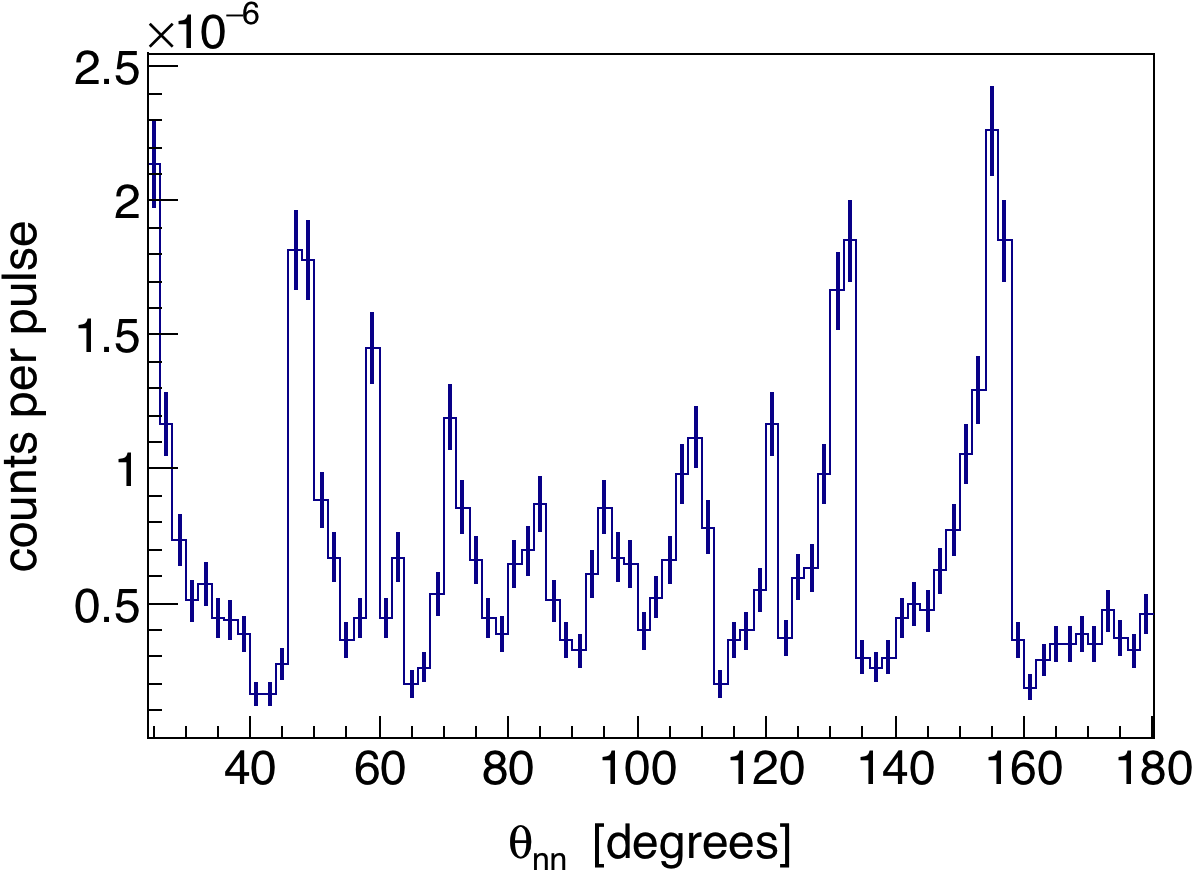
\includegraphics[width=0.9\textwidth]{Content/Methods/DetAcceptance.png}
\caption{Raw n-n opening angle measurement from the photofission of $^{238}$U. 
This distribution is highly influenced by the detection system's geometry and efficiency.
}
\label{fig:DetAcceptance}
\end{figure}

The construction of $nn_{\text{uncorr}}(\theta)$ is achieved by examining pulses in pairs of two, under the requirement that both pulses occurred within 0.2 seconds of each other in order to increase the chance that they occurred under the same experimental conditions.
For each pulse-pair that has two neutron events in both pulses, all possible pairs of uncorrelated neutrons are examined (a total of 4 in this case), and the opening angle of each uncorrelated neutron-neutron (n-n) pair is calculated.

Figure~\ref{fig:SPDPNormalization}(a) shows the measured $nn_{\text{corr}}(\theta)$ yield distribution of neutrons from the photofission of $^{238}$U.
The structure seen here is reflective of the underlying n-n angular correlations as well as the geometric acceptance and efficiencies of the neutron detectors.
Figure~\ref{fig:SPDPNormalization}(b) reveals how a clear picture of n-n correlations emerges when taking the ratio between $nn_{\text{corr}}(\theta)$ and $nn_{\text{uncorr}}(\theta)$.
\begin{figure}[]
\centering
    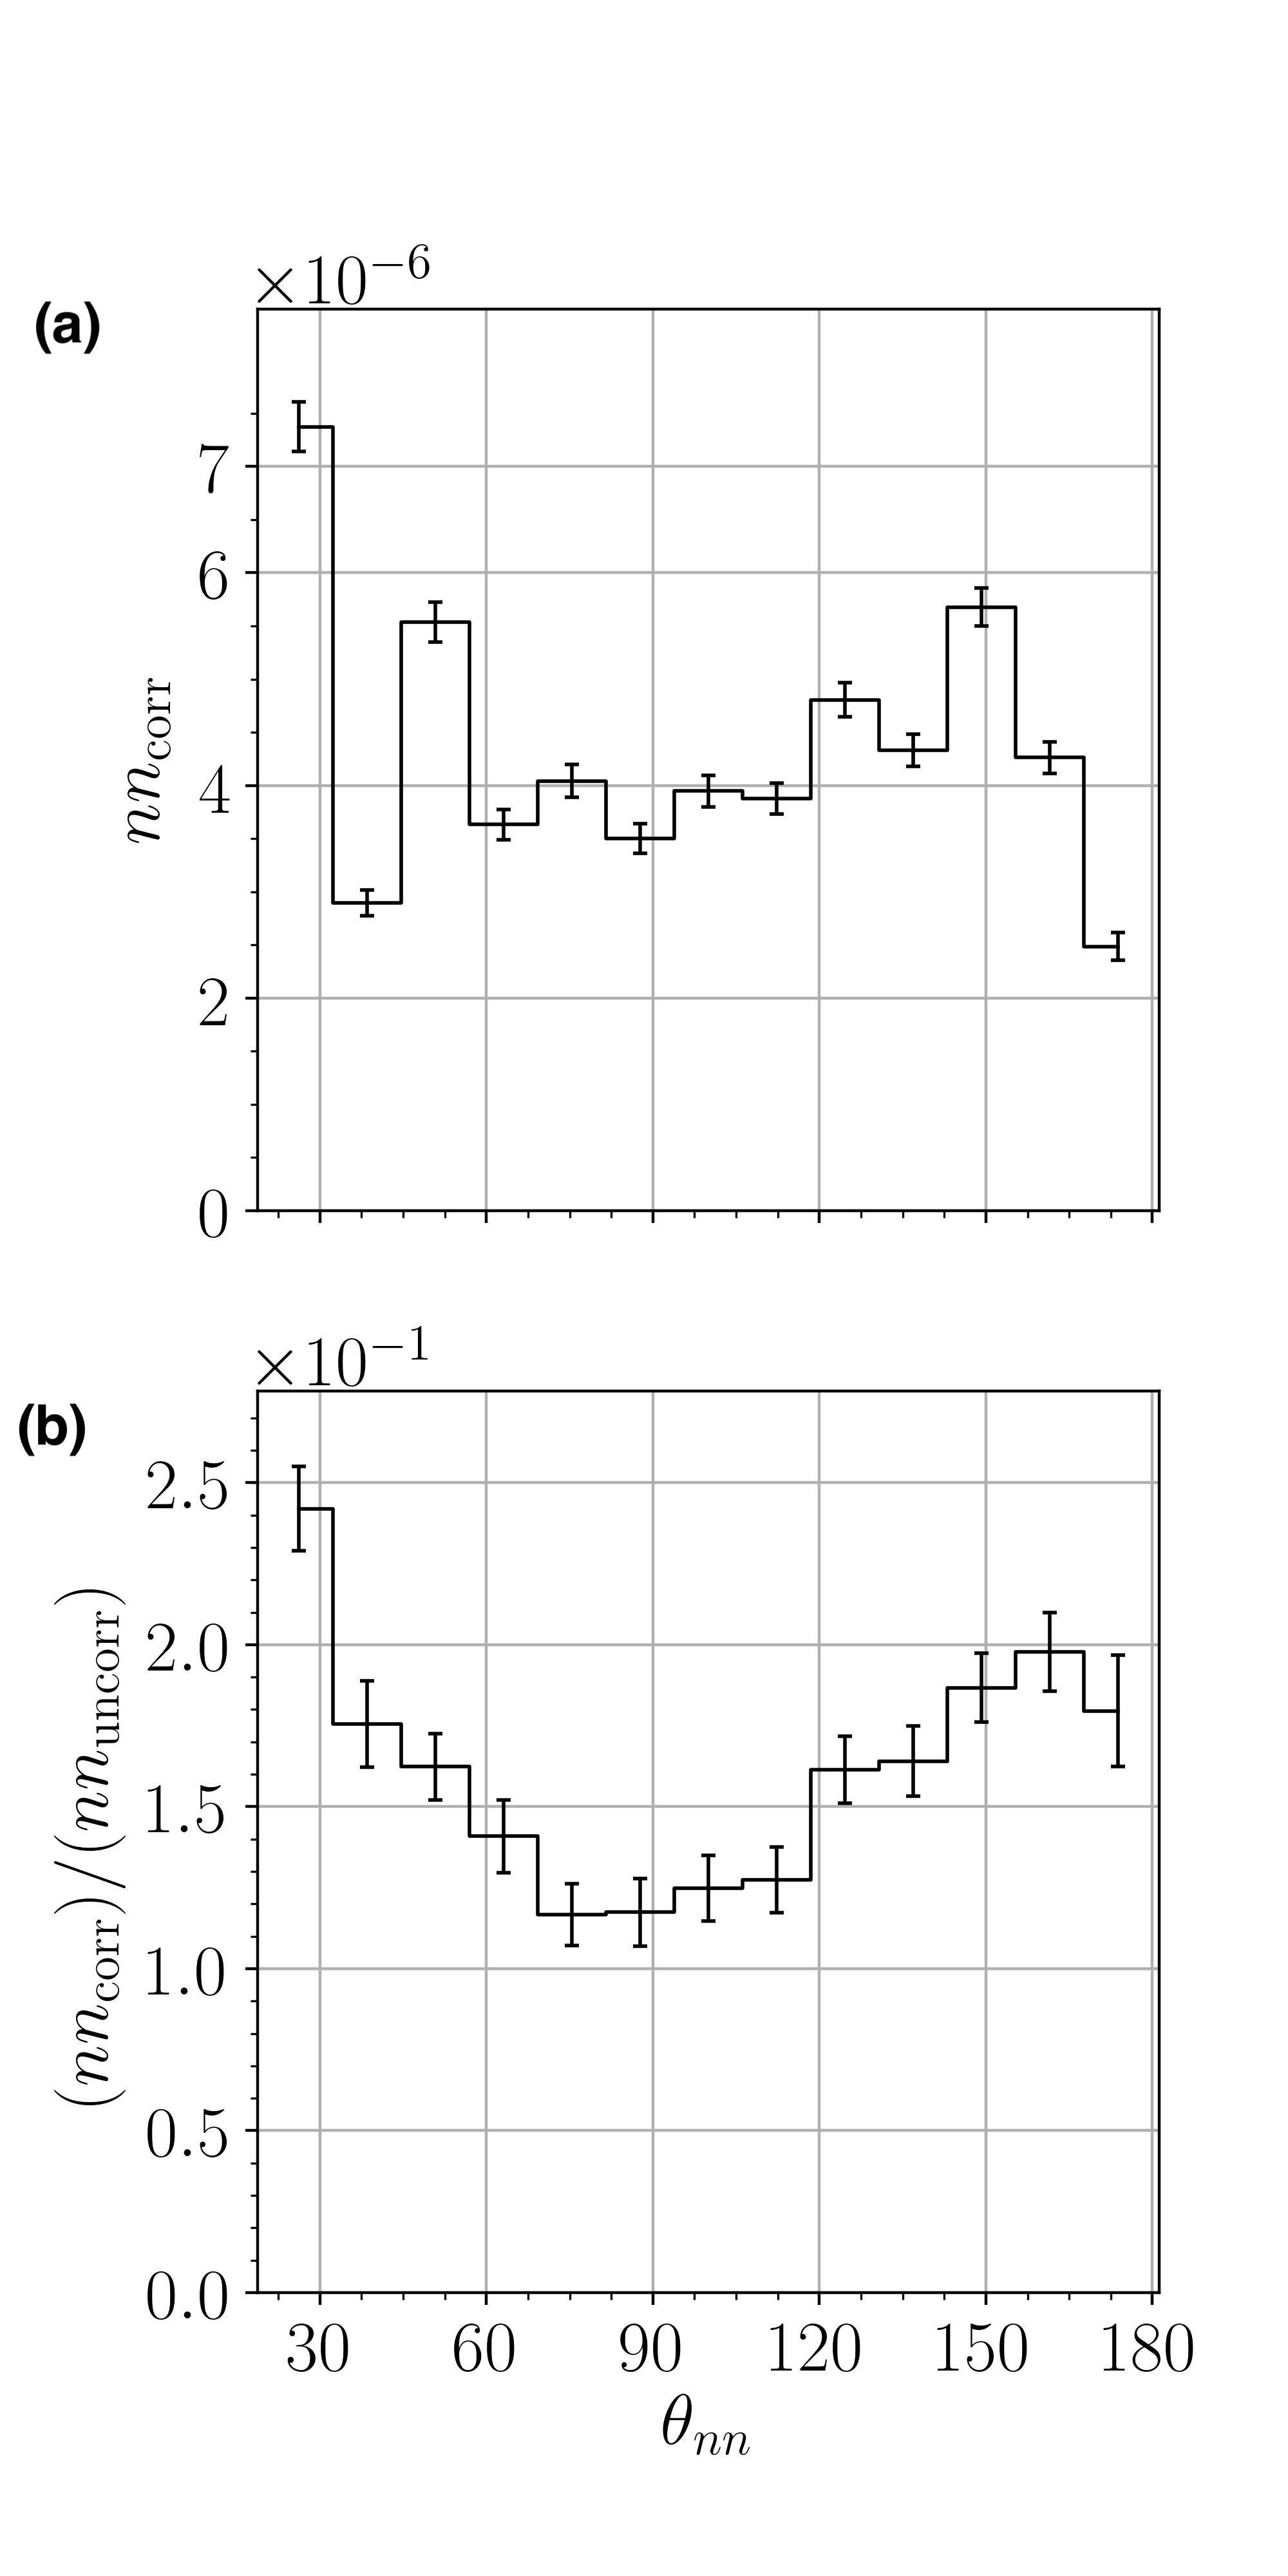
\includegraphics[width=0.7\textwidth]{Content/Methods/SPDPNormalization.png}
    \caption{(a) n-n opening angle distribution from the photofission of $^{238}$U before normalization, and, (b) after normalizing to the distribution of uncorrelated n-n events from different pulses.
    All measured neutrons have an energy greater than 0.4 MeV.}
    \label{fig:SPDPNormalization}
\end{figure}

In order to effectively minimize the dependence of the result on detector geometry/efficiency, the numerator and denominator of Eq.~\ref{eq:angularCorr} must comprise neutron pairs with a similar energy distribution.
This is the reason for using only pulse-pairs that have two events in each pulse, as it increases the percentage of pulse-pairs comprising coincident neutrons from fission as opposed to accidental coincident neutrons from $(\gamma,n)$.
Neutrons from fission and $(\gamma,n)$ have different energy distributions, and note that the detection of multiple neutrons from $(\gamma,n)$ are completely removed from $nn_{\text{corr}}(\theta)$, the numerator in Eq.~\ref{eq:angularCorr}, by the subtraction of accidental coincidences.

When examining differences between the neutron energy distributions in $nn_{\text{corr}}(\theta)$ and $nn_{\text{uncorr}}(\theta)$, it is important to consider how the energies of both neutrons forming n-n pairs vary together, or, in other words, their joint energy distribution.
Fig.~\ref{fig:ErgDiffLego} shows the ratio between the rates for correlated and uncorrelated n-n pairs of various binned energies.
The effect that these discrepancies in energy distribution have on the final result can be examined by applying a weighting factor to each event in $nn_{\text{uncorr}}(\theta)$ such that a recalculation of the result in Fig.~\ref{fig:ErgDiffLego} produces a flat curve.
A comparison of the determined angular correlation with and without the application of these weighting factors to all uncorrelated n-n events is seen in Fig.~\ref{fig:WeightedErgDiff}.
The resulting differences in angular correlation are negligible.
\begin{figure}[]
\centering
    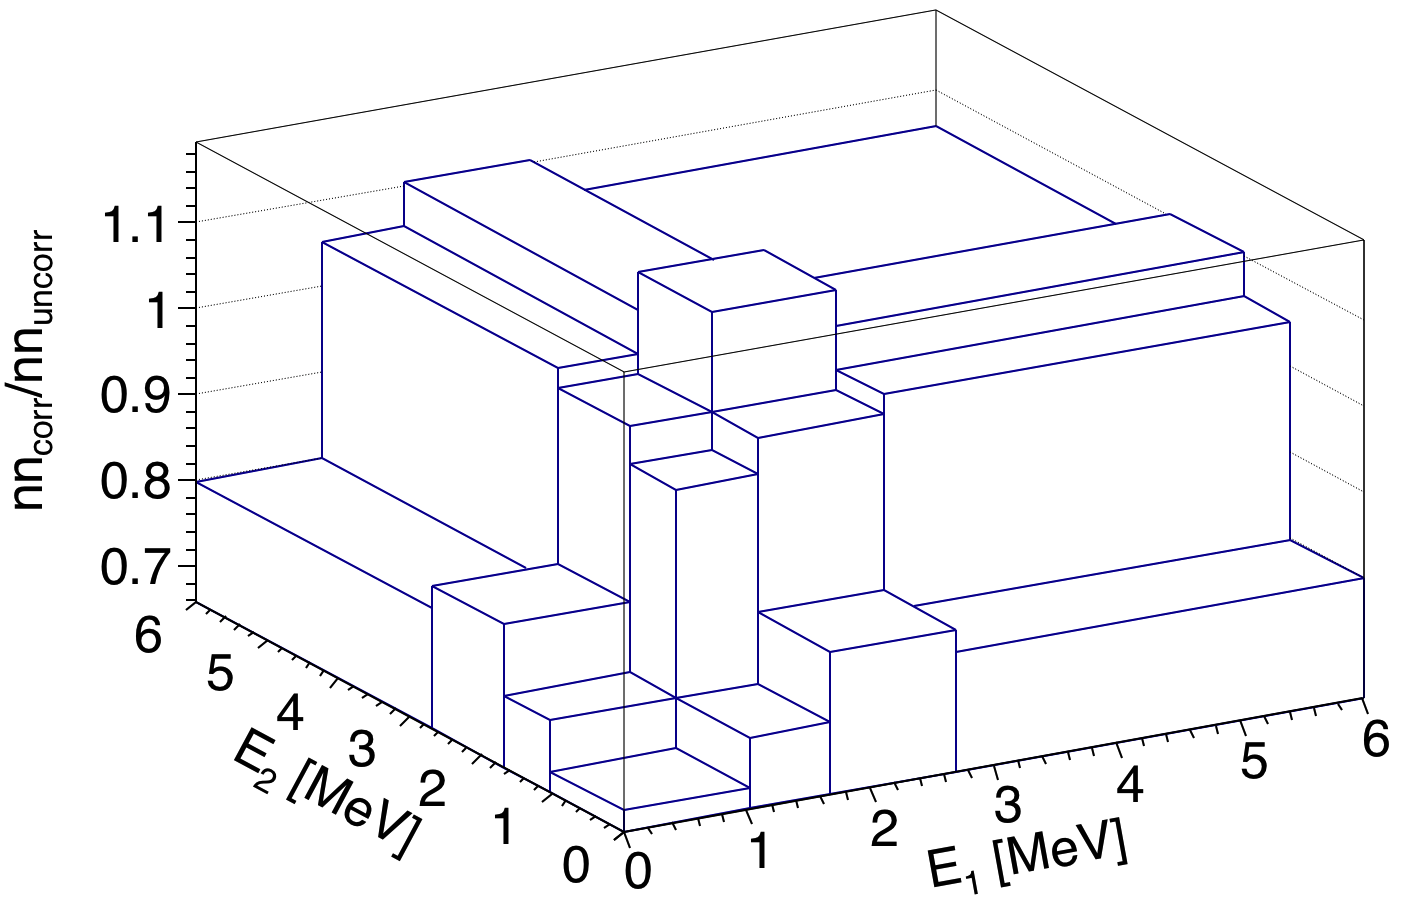
\includegraphics[width=0.45\textwidth]{Content/Methods/ErgDiffLego.png}
    \caption{
    The z-axis represents the ratio between the correlated and uncorrelated rates of binned n-n energies.
    The energy bins are chosen such that each contains an equal number of events, or 1/16th of the total events.
    }
    \label{fig:ErgDiffLego}
\end{figure}
\begin{figure}[]
\centering
    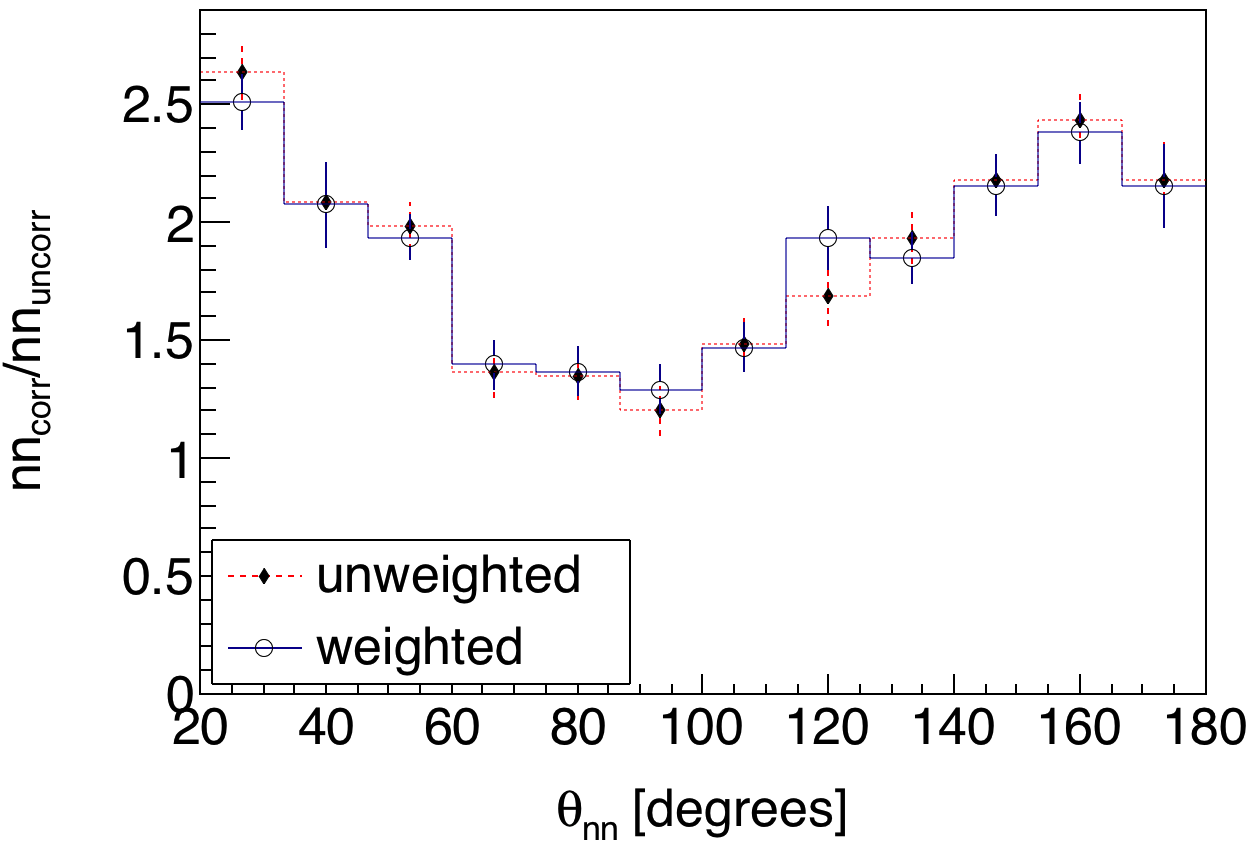
\includegraphics[width=0.45\textwidth]{Content/Methods/WeightedErgDiff.png}
    \caption{
Each uncorrelated n-n event can be weighted such that the weighted histograms of the joint n-n energy distributions of correlated and uncorrelated n-n pairs are equal.
Comparison of the calculated angular correlation results, with and without such weighting factors applied to all uncorrelated n-n events, illustrates that any effects due to the discrepancies in the joint energy distributions of correlated and uncorrelated n-n pairs are negligible.
    }
    \label{fig:WeightedErgDiff}
\end{figure}

The angular correlation of neutron coincidences from the photo-disintegration of D$_{2}$O was measured, producing a flat angular correlation as expected (see Fig.~\ref{fig:D2Otheta_nn}).
A cylindrical bottle with a height of 4.5~cm and a radius of 1~cm was filled with heavy water 
(D$_{2}$O) and subject to the bremsstrahlung photon beam, producing neutron coincidences at a rate of 1.4$\times10^{-4}$ per pulse.
The photo-disintegration of the deuteron, which produces only uncorrelated neutrons, is the only neutron producing reaction involved because the bremsstrahlung endpoint was below the $(\gamma, 1n)$ threshold of $^{16}$O.
\begin{figure}[h]
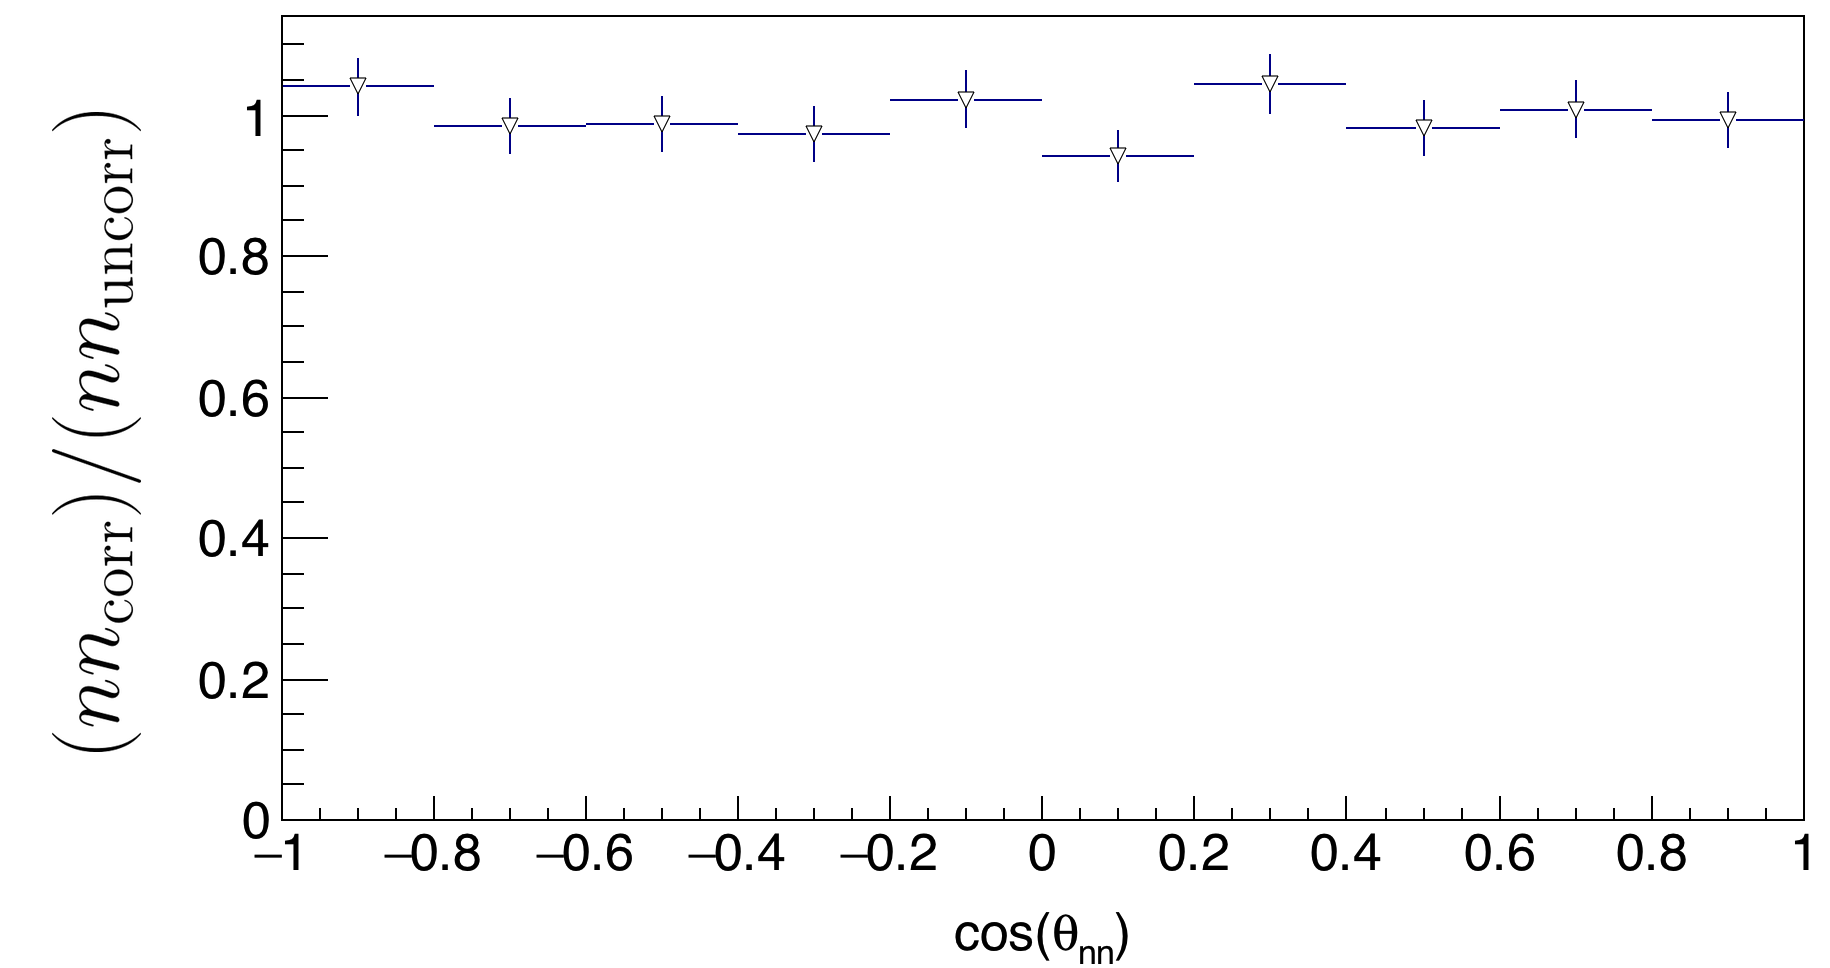
\includegraphics[width=0.9\textwidth]{Content/Methods/D2Otheta_nn.png}
\caption{The opening angle distribution of neutrons from the photo-disintegration of D$_{2}$O is uniform.
This is expected because the photo-disintegration of D$_{2}$O emits only a single neutron, and thus this distribution arises solely from neutron accidentals.}
\label{fig:D2Otheta_nn}
\end{figure}

\FloatBarrier
\subsection{Subtraction of Accidental Coincidences}
\label{Reconstruction of Accidental Coincidence}
The detection of two uncorrelated events in coincidence, whether caused by neutrons, photons, or noise, is referred to as an \emph{accidental coincidence}, or just \emph{accidental} for short.
A small number of accidental photon events will exist in the neutron time of flight range because of the smearing of the gamma flash.
There are also accidentals due to noise, which can be estimated with a non-neutron producing target made from aluminum (see Fig.~\ref{fig:Noise}).
The accelerator's current was adjusted so that there are, on average, less than 1.0 fissions per accelerator pulse, but nevertheless, statistical fluctuations in the number of fissions per pulse result in accidental coincident neutrons that originated from different, and therefore, uncorrelated fissions.
There are also uncorrelated neutrons produced when multiple $(\gamma, n)$ reactions occur in a single pulse.

The $^{238}$U cross-section of $(\gamma, n)$, integrated over the relevant bremsstrahlung energy distribution, is about a factor of 5.5 times greater than it is for photofission (see Fig.~\ref{fig:CrossSection}).
As a result, the raw neutron coincidence data will contain a significant number of neutron coincidences from multiple $(\gamma, n)$ reactions in relation to neutron coincidences from fission.
If accidentals were not subtracted from the result, then they would tend to wash out the signal from correlated neutrons. 
\begin{figure}[]
\centering
    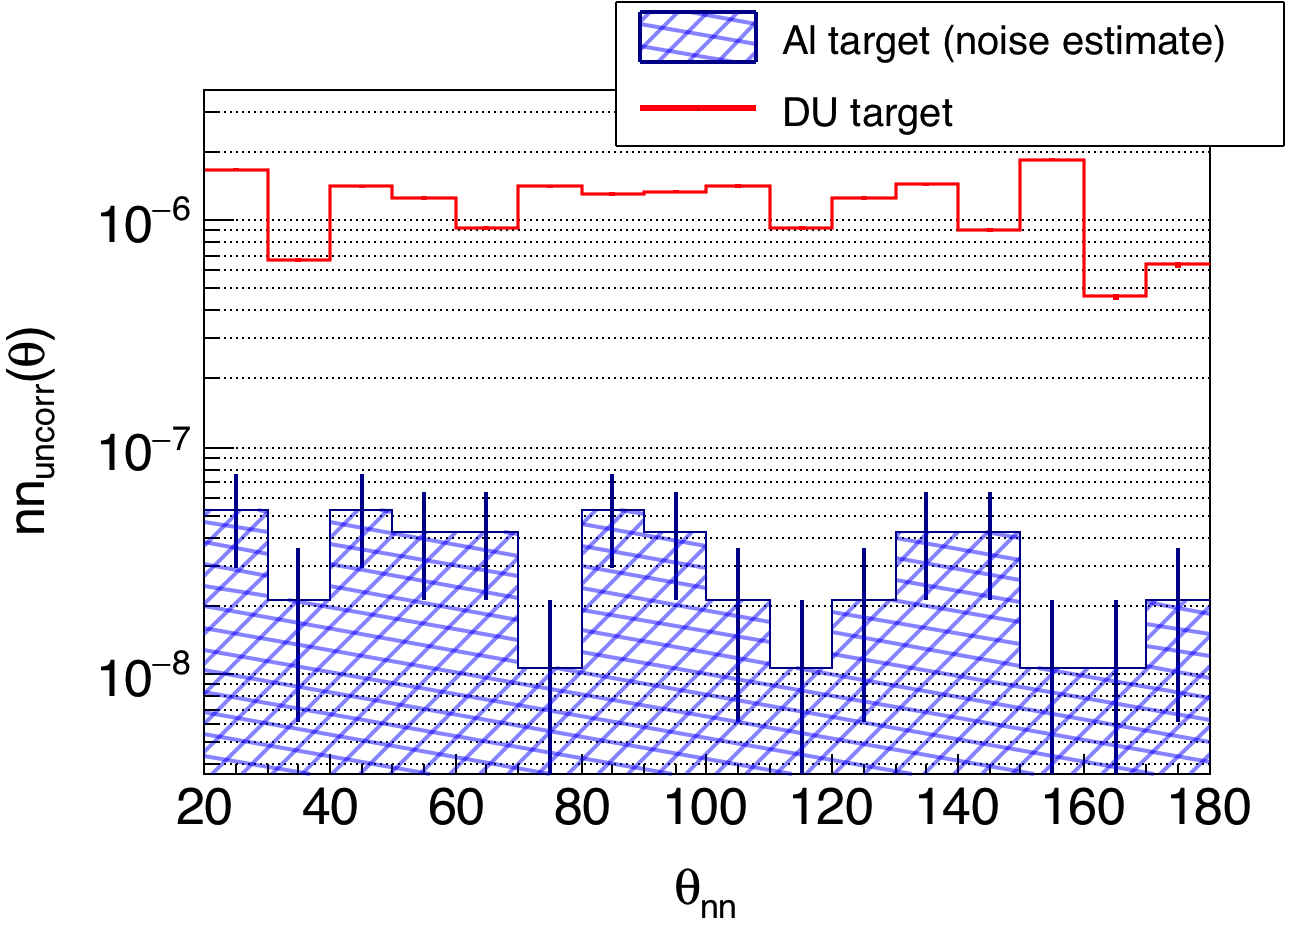
\includegraphics[width=0.8\textwidth]{Content/Methods/Noise.png}
    \caption{An Al target was designed to scatter the same number of photons as the DU target, thus serving as an equivalent non-neutron producing target well-suited for noise estimates.
    The rate of coincident events for the Al target is 3\% that of the DU target. 
        }
    \label{fig:Noise}
\end{figure}
\begin{figure}[]
\centering
    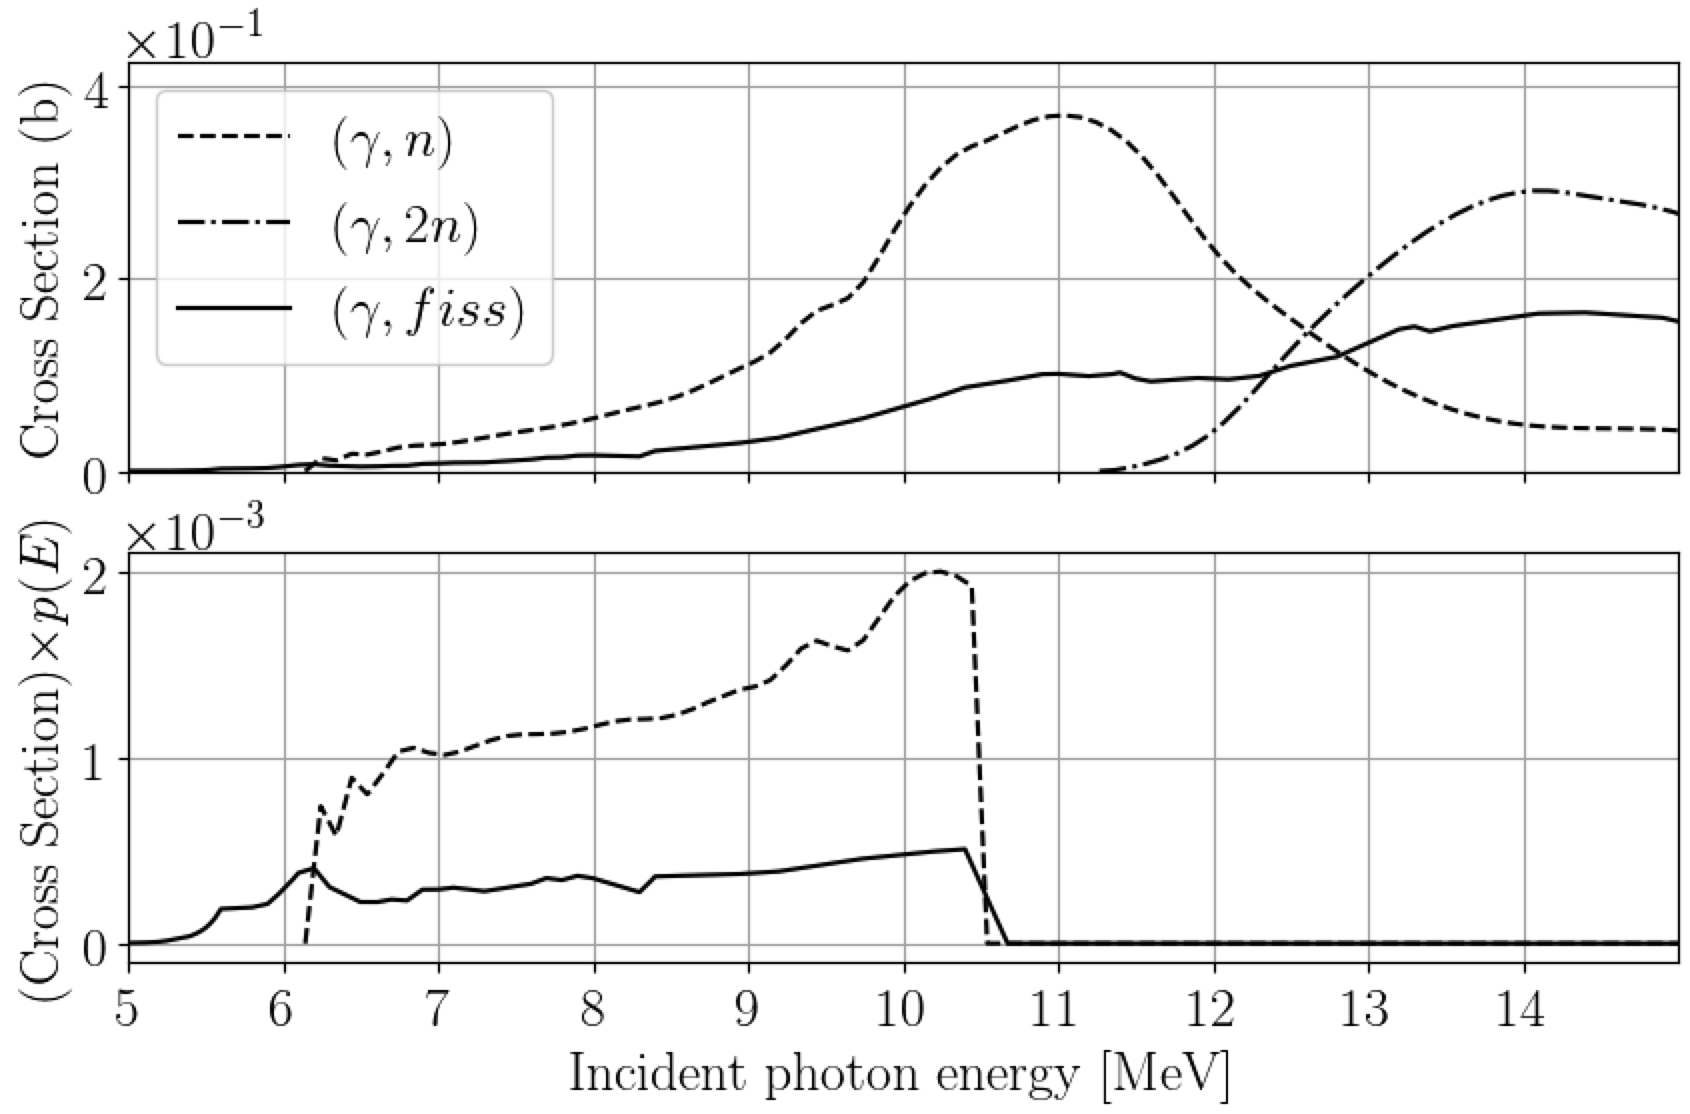
\includegraphics[width=0.95\textwidth]{Content/Methods/CrossSections.png}
    \caption{(top) ENDF cross-sections of $(\gamma$,fiss), direct $(\gamma$,n), and direct $(\gamma$,2n).
    (bottom) Cross-sections weighted by the simulated relative rate of bremsstrahlung photons that reach the target as a function of photon energy. The integrated cross-sections of $(\gamma, n)$ is 5.5 times greater than for $(\gamma, \text{fiss})$. }
    \label{fig:CrossSection}
\end{figure}
\begin{figure}[]
\centering
    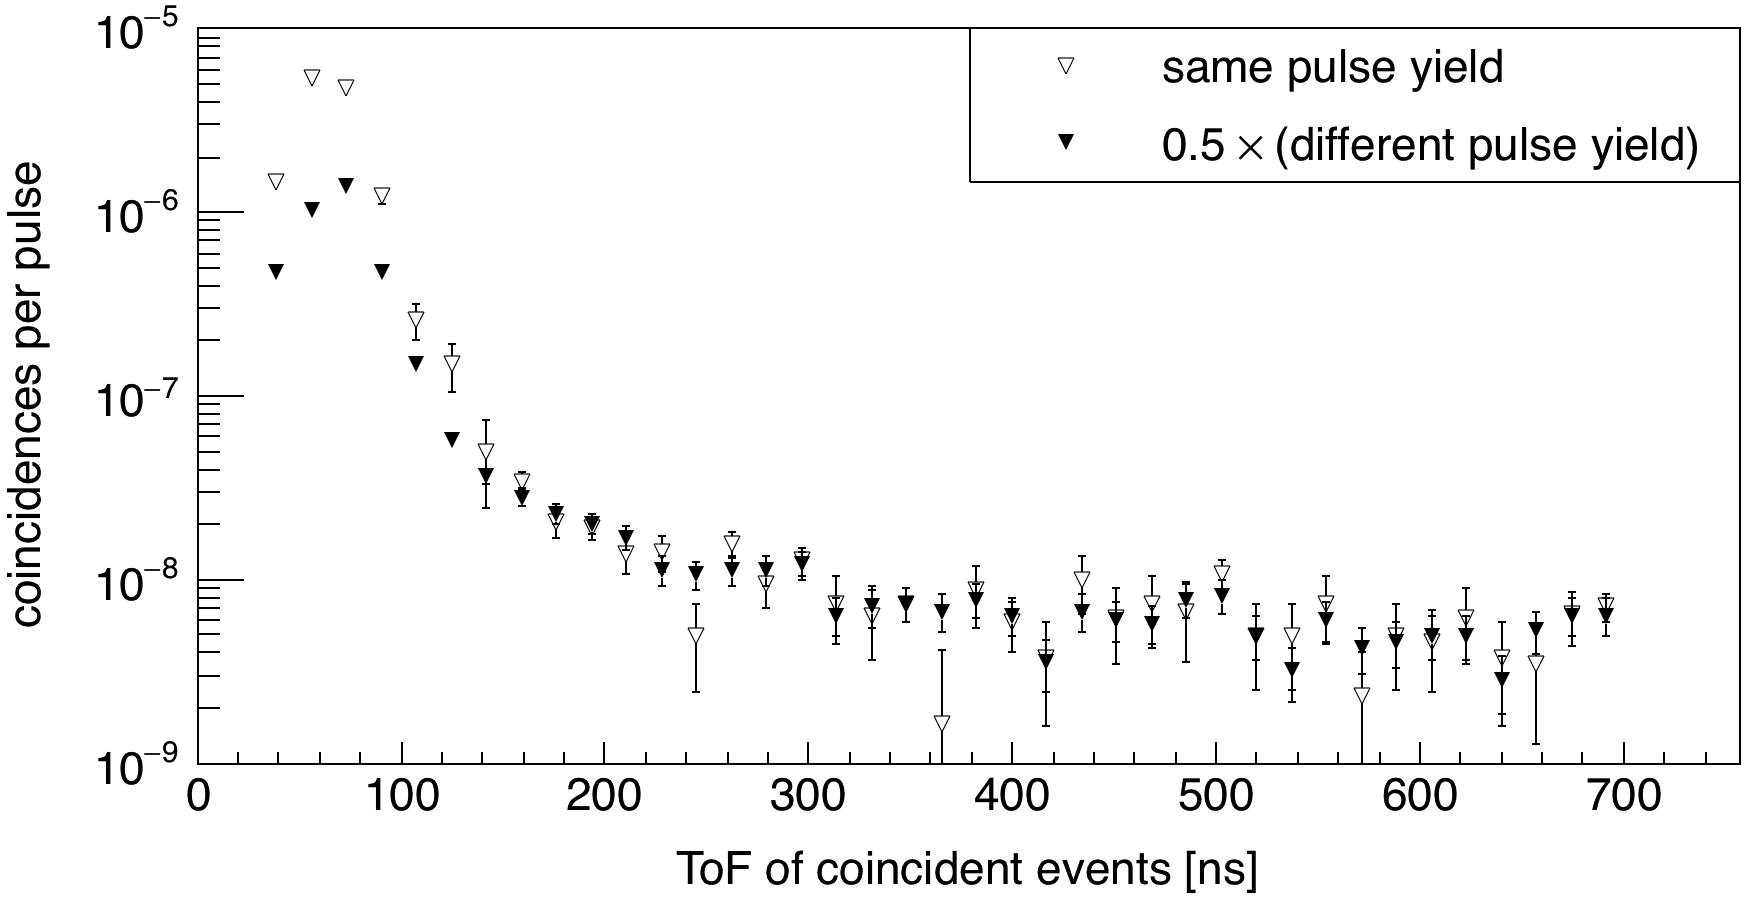
\includegraphics[width=0.9\textwidth]{Content/Methods/NoiseSubtraction.png}
    \caption{The different pulse yield captures the effects of noise due to accidentals.
    The y-axis represents the number of coincidences in which both events had a ToF within a given 20~ns wide bin.
    Because events with a ToF above 120~ns are predominately due to noise, which correspond to a 0.5 MeV neutron, the same pulse yield is equal to 1/2 times the different pulse yield.
    }
    \label{noise_siubtraction}
\end{figure}

The raw measurement consists of a mix of correlated and accidental neutron coincidences, that is
\begin{equation}
\label{eq:corr_uncorr}
nn_{\text{raw}}(\theta)= nn_{\text{corr}}(\theta) + nn_{\text{acc}}(\theta) \, ,
\end{equation}
where $nn_{\text{raw}}(\theta)$ and $nn_{\text{acc}}(\theta)$ are the rates, per pulse, of the detection of neutron pairs with opening angle of $\theta$ for all events and for accidental coincident events, respectively.

Because accidental coincidences consist of two independent events, it does not matter whether these two events occurred during the same pulse or during different pulses, given that the two different pulses occurred at around the same time and thus under the same experimental conditions.
Therefore, $nn_{\scaleto{DP}{4pt}}(\theta)$, the distribution from different-pulse neutron events, is proportional to $nn_{\text{acc}}(\theta)$.
In other words,  $nn_{\scaleto{DP}{4pt}}(\theta)$ and $nn_{\text{acc}}(\theta)$ have the same shape.
However, $nn_{\text{acc}}(\theta)$ is not equal to $nn_{\scaleto{DP}{4pt}}(\theta)$, because there are, on average, twice as many events in a pulse-pair than there are in a single pulse.
For this reason, as the following analysis shows,~$nn_{\text{acc}}(\theta) = \frac{1}{2}nn_{\scaleto{DP}{4pt}}(\theta)$.

The number of uncorrelated events detected per pulse is assumed to follow the Poissonian distribution, which describes the occurrence of independent random events.
Let $\lambda$ represent the mean number of uncorrelated events per pulse.
The total per-pulse accidental coincidence frequency for single pulses, denoted by $\sum_{\theta} nn_{\text{acc}}(\theta)$, is equal to the Poissonian probability of there being exactly two events detected in a single pulse\footnote{For the sake of brevity, cases of greater than two-fold coincidence are not considered in this analysis, as it is not necessary because of the low detection rates during this work.
It can be shown, however, that accounting for any number of coincidences, from zero all the way up to $\infty$-fold coincident events in a pulse or pulse-pair, will give the same answer.}:
\begin{equation} \label{math:SP}
    \begin{split}
    \sum_{\theta} nn_{\text{acc}}(\theta) & = \frac{e^{-\lambda}\lambda^{2}}{2!} \\
        &\approx \frac{\lambda^2}{{2}} + \mathcal{O}(\lambda^3) \, .
    \end{split}
\end{equation}
To determine the value of $\lambda$, one would need the ability to distinguish between true and accidental coincidences, as $\lambda$ refers only to the rate of accidental coincidences.
Such information is not known, but the largest possible value for $\lambda$ is the mean number of events per pulse, as this assumes that all events are uncorrelated.
For this work, this places an upper bound on $\lambda$ of $3\times 10^{-6}$, which is small enough to neglect all terms on the order of $\lambda^3$ or greater.

For the case of different-pulse pairs, a ``coincidence'' is said to occur when there is an event in both pulses.
The total per-pulse-pair coincidence frequency is the square of the Poissonian probability of there being one event in a single pulse, since a pulse-pair coincidence consists of two neutron events, one in each pulse.
Cases in which there are more than two events in a given pulse are neglected here because they occur at a rate that is a factor of 100 times less than the rate of pulses with only a single event.
The total per-pulse-pair coincidence frequency, $\sum_{\theta} nn_{\scaleto{DP}{4pt}}(\theta)$, is given by 
\begin{equation} \label{math:DP}
    \begin{split}
   \sum_{\theta} nn_{\scaleto{DP}{4pt}}(\theta)&= \left(e^{-\lambda}\lambda\right)^{2} \\
    &\approx \lambda^2 + \mathcal{O}(\lambda^3) \, .
    \end{split}
\end{equation}
For the reasons explained above, $nn_{\scaleto{DP}{4pt}}(\theta)$ and $nn_{\text{acc}}(\theta)$ have the same shape, thus, from Eq.'s (\ref{math:DP}) and (\ref{math:SP}) it follows that 
\begin{equation}
\label{eq:uncorr_DP}
nn_{\text{acc}}(\theta) = \frac{1}{2}nn_{\scaleto{DP}{4pt}}(\theta) \,.
\end{equation}

